\PassOptionsToPackage{dvipsnames,svgnames,x11names}{xcolor}
\documentclass[tikz,border=8pt]{standalone}
\usetikzlibrary{arrows.meta,positioning,calc,shapes,shadows,decorations.pathmorphing,shapes.geometric,backgrounds,decorations.markings,decorations.pathreplacing,decorations.text,fit,shapes.misc,shapes.arrows,matrix,bending,3d,chains,intersections,shapes.symbols,svg.path,shapes.multipart,snakes,shapes.callouts,angles,quotes}
\providecolor{gold}{RGB}{212,175,55}
\providecolor{silver}{RGB}{192,192,192}
\providecolor{bronze}{RGB}{205,127,50}
\providecolor{darkblue}{RGB}{0,0,139}
\providecolor{lightblue}{RGB}{173,216,230}
\providecolor{darkgreen}{RGB}{0,100,0}
\providecolor{lightgreen}{RGB}{144,238,144}
\providecolor{darkred}{RGB}{139,0,0}
\providecolor{navy}{RGB}{0,0,128}
\providecolor{skyblue}{RGB}{135,206,235}
\providecolor{beige}{RGB}{245,245,220}
\providecolor{cream}{RGB}{255,253,208}
\usepackage{amsmath}
\usepackage{amssymb}
\usepackage{fontawesome5}
\usetikzlibrary{fadings,shadows.blur,patterns,patterns.meta}

% --- Custom Color Palette ---
\definecolor{codebg}{RGB}{40, 44, 52}
\definecolor{codeheader}{RGB}{33, 37, 43}
\definecolor{codefg}{RGB}{171, 178, 191}
\definecolor{greenstr}{RGB}{152, 195, 121}
\definecolor{redtag}{RGB}{224, 108, 117}
\definecolor{attrcolor}{RGB}{209, 154, 102}

\definecolor{mandcolor}{RGB}{190, 20, 50}      % Mandatory Crimson Red
\definecolor{condcolor}{RGB}{30, 55, 95}       % Routing Engine Navy Blue
\definecolor{condborder}{RGB}{45, 80, 140}
\definecolor{cropcolor}{RGB}{115, 40, 155}     % Art Direction Purple
\definecolor{chassisbg}{RGB}{242, 245, 250}
\definecolor{chassisborder}{RGB}{175, 190, 210}

% Device Frame Colors
\definecolor{devicebody}{RGB}{225, 229, 235}
\definecolor{deviceborder}{RGB}{165, 175, 188}
\definecolor{screenbg}{RGB}{248, 250, 252}

% Mac Window Controls
\definecolor{macred}{RGB}{255, 95, 86}
\definecolor{macyellow}{RGB}{255, 189, 46}
\definecolor{macgreen}{RGB}{39, 201, 63}

\begin{document}
\begin{tikzpicture}[
    condbox/.style={
        draw=condborder,
        fill=white,
        line width=1.5pt,
        rounded corners=6pt,
        minimum width=5.6cm,
        minimum height=1.5cm,
        text width=5.2cm,
        align=center,
        blur shadow={shadow opacity=18, shadow yshift=-2pt, shadow blur radius=4pt}
    },
    bubble/.style={
        draw=mandcolor!60,
        fill=mandcolor!4,
        line width=1.2pt,
        rounded corners=8pt,
        text width=24cm,
        inner sep=16pt,
        align=justify,
        font=\normalsize\sffamily,
        blur shadow={shadow opacity=12, shadow yshift=-2pt, shadow blur radius=4pt}
    },
    true_arrow/.style={
        -Stealth=3mm,
        line width=3.8pt,
        draw=mandcolor
    },
    flow_arrow/.style={
        -Stealth=3mm,
        line width=2.2pt,
        draw=condborder,
        shorten >= 3pt,
        shorten <= 3pt
    },
    ribbon/.style={
        line width=2pt,
        draw=condborder!75,
        dashed
    }
]

% -------------------------------------------------------------------------
% 1. Global Canvas Background (Pure White)
% -------------------------------------------------------------------------
\fill[white] (-15, -14.0) rectangle (15, 13.5);

% -------------------------------------------------------------------------
% 2. Headers
% -------------------------------------------------------------------------
\node[font=\Huge\bfseries\sffamily\color{mandcolor}] at (0,12.3804) {\texttt{<picture>}: The Mandatory "Directive"};
\node[font=\Large\sffamily\bfseries\color{gray!80!black}] at (0,11.3804) {Art Direction: The Browser is Stripped of Autonomy};

% -------------------------------------------------------------------------
% 3. macOS-Style Code Editor Window & Logical Ribbons (Left Column)
% -------------------------------------------------------------------------
% Window Outer Container with Drop Shadow
\draw[draw=black!40, fill=codebg, line width=1pt, rounded corners=8pt, blur shadow={shadow opacity=25, shadow yshift=-3pt, shadow blur radius=6pt}] (-13.5, 2.0) rectangle (-5.5, 9.5);

% Window Title Bar
\path[fill=codeheader, rounded corners=8pt] (-13.5, 8.8) rectangle (-5.5, 9.5);
\fill[codeheader] (-13.5, 8.8) rectangle (-5.5, 9.0);
\draw[draw=black!50, line width=0.75pt] (-13.5, 8.8) -- (-5.5, 8.8);

% Window Control Dots
\fill[macred] (-13.0, 9.15) circle (3.2pt);
\fill[macyellow] (-12.5, 9.15) circle (3.2pt);
\fill[macgreen] (-12.0, 9.15) circle (3.2pt);
\node[font=\tiny\ttfamily\color{codefg!70}, anchor=center] at (-9.5, 9.15) {index.html};

% Code Snippet Content with Precise Line Anchoring
\node[anchor=west, font=\ttfamily\footnotesize, text=codefg, inner sep=0pt] at (-13.0, 8.2) {<\textcolor{redtag}{picture}>};

% Node L1: 1024px source at y = 7.0
\node[anchor=west, align=left, font=\ttfamily\footnotesize, text=codefg, inner sep=0pt] (codeL1) at (-12.7, 7.0) {
    <\textcolor{redtag}{source} \textcolor{attrcolor}{media}=\textcolor{greenstr}{"(min-width: 1024px)"}\\
    \hspace*{5mm}\textcolor{attrcolor}{srcset}=\textcolor{greenstr}{"wide-crop.jpg"}>
};

% Node L2: 768px source at y = 5.0
\node[anchor=west, align=left, font=\ttfamily\footnotesize, text=codefg, inner sep=0pt] (codeL2) at (-12.7, 5.0) {
    <\textcolor{redtag}{source} \textcolor{attrcolor}{media}=\textcolor{greenstr}{"(min-width: 768px)"}\\
    \hspace*{5mm}\textcolor{attrcolor}{srcset}=\textcolor{greenstr}{"square-crop.jpg"}>
};

% Node L3: img fallback at y = 3.0
\node[anchor=west, align=left, font=\ttfamily\footnotesize, text=codefg, inner sep=0pt] (codeL3) at (-12.7, 3.0) {
    <\textcolor{redtag}{img} \textcolor{attrcolor}{src}=\textcolor{greenstr}{"portrait-crop.jpg"} \textcolor{attrcolor}{alt}=\textcolor{greenstr}{"Cat"}>
};

\node[anchor=west, font=\ttfamily\footnotesize, text=codefg, inner sep=0pt] at (-13.0, 2.35) {<\textcolor{redtag}{/picture}>};

% Developer's Orders Label
\node[font=\small\bfseries\sffamily\color{gray!80!black}, text width=5.5cm, align=center] at (-9.5, 1.0) {Developer's Strict Orders\\(Top-to-Bottom Execution)};

% -------------------------------------------------------------------------
% 4. Hard Routing Engine Chassis (Center Column)
% -------------------------------------------------------------------------
% Panel Background Box
\draw[draw=chassisborder, line width=1.5pt, left color=chassisbg, right color=chassisbg!65!white, rounded corners=10pt, blur shadow={shadow opacity=20, shadow yshift=-3pt, shadow blur radius=6pt}] (-3.0, -7.0) rectangle (3.0, 10.0);

% Chassis Header Accent & Status Indicators
\path[fill=condcolor!10, rounded corners=10pt] (-3.0, 9.2) rectangle (3.0, 10.0);
\fill[condcolor!10] (-3.0, 9.2) rectangle (3.0, 9.4);
\draw[draw=chassisborder!80, line width=0.75pt] (-3.0, 9.2) -- (3.0, 9.2);

\node[font=\normalsize\bfseries\sffamily\color{condcolor}, anchor=west] at (-2.7, 9.6) {\faProjectDiagram\ Hard Routing Engine};
\fill[condcolor!60] (2.4, 9.6) circle (2.5pt);
\fill[green!70!black] (2.8, 9.6) circle (2.5pt);

% Condition 1 Box (Center at 0, 8.0)
\node[condbox] (cond1) at (0, 8.0) {
    \textbf{\sffamily IF} Media\\
    \texttt{(min-width: 1024px)}\\[1.5mm]
    \footnotesize\sffamily Evaluates to \textbf{\color{condcolor}TRUE}?
};

% Condition 2 Box (Center at 0, 1.5)
\node[condbox] (cond2) at (0, 1.5) {
    \textbf{\sffamily ELSE IF} Media\\
    \texttt{(min-width: 768px)}\\[1.5mm]
    \footnotesize\sffamily Evaluates to \textbf{\color{condcolor}TRUE}?
};

% Condition 3 Box (Center at 0, -5.0)
\node[condbox] (cond3) at (0, -5.0) {
    \textbf{\sffamily ELSE} (Fallback \texttt{<img>})\\[1.5mm]
    \footnotesize\sffamily Always \textbf{\color{condcolor}TRUE}
};

% -------------------------------------------------------------------------
% 5. Routing Flow & Connectors
% -------------------------------------------------------------------------
% Logical Ribbons (Code Line to Routing Evaluation Box)
\draw[ribbon, -{Circle[length=3.5pt]}] (-5.5, 7.0) .. controls (-4.25, 7.0) and (-4.25, 8.0) .. (-3.0, 8.0);
\draw[ribbon, -{Circle[length=3.5pt]}] (-5.5, 5.0) .. controls (-4.25, 5.0) and (-4.25, 1.5) .. (-3.0, 1.5);
\draw[ribbon, -{Circle[length=3.5pt]}] (-5.5, 3.0) .. controls (-4.25, 3.0) and (-4.25, -5.0) .. (-3.0, -5.0);

% FALSE Paths (Vertical Blue Arrows)
\draw[flow_arrow] (cond1.south) -- (cond2.north) node[midway, right=6pt, font=\footnotesize\bfseries\sffamily, color=condborder] {FALSE (Skip)};
\draw[flow_arrow] (cond2.south) -- (cond3.north) node[midway, right=6pt, font=\footnotesize\bfseries\sffamily, color=condborder] {FALSE (Skip)};

% TRUE Paths (Horizontal Red Arrows)
\draw[true_arrow] (cond1.east) -- (6.6, 8.0)
    node[midway, above=8pt, font=\footnotesize\bfseries\sffamily, color=mandcolor] {MUST EXECUTE}
    node[midway, below=8pt, font=\scriptsize\sffamily, color=mandcolor] {(Ignores Cache/Network)};

\draw[true_arrow] (cond2.east) -- (6.6, 1.5)
    node[midway, above=8pt, font=\footnotesize\bfseries\sffamily, color=mandcolor] {MUST EXECUTE}
    node[midway, below=8pt, font=\scriptsize\sffamily, color=mandcolor] {(Ignores Cache/Network)};

\draw[true_arrow] (cond3.east) -- (6.6, -5.0)
    node[midway, above=8pt, font=\footnotesize\bfseries\sffamily, color=mandcolor] {MUST EXECUTE}
    node[midway, below=8pt, font=\scriptsize\sffamily, color=mandcolor] {(Ignores Cache/Network)};

% -------------------------------------------------------------------------
% 6. Target Hardware Device Mockups (Right Column)
% -------------------------------------------------------------------------

% --- Device 1: Desktop Monitor (16:9 Screen, Center x=9.5) ---
% Stand & Base
\fill[deviceborder!90] (8.8, 5.45) rectangle (10.2, 5.6);
\fill[deviceborder] (9.35, 5.6) rectangle (9.65, 6.0);

% Monitor Outer Frame (Width 5.4cm, Height 4.0cm: 6.8, 6.0 to 12.2, 10.0)
\draw[draw=deviceborder, fill=devicebody, line width=1.2pt, rounded corners=5pt, blur shadow={shadow opacity=16, shadow yshift=-2pt, shadow blur radius=4pt}] (6.8, 6.0) rectangle (12.2, 10.0);

% Inner Screen (7.2, 6.4 to 11.8, 9.6)
\draw[draw=black!60, fill=screenbg, line width=1pt] (7.2, 6.4) rectangle (11.8, 9.6);

% Artwork Division (Upper Zone: y = 8.0 to 9.6)
\begin{scope}
    \clip (7.2, 8.0) rectangle (11.8, 9.6);
    \fill[cropcolor!12] (7.2, 8.0) rectangle (11.8, 9.6);
    \draw[draw=cropcolor!30, fill=cropcolor!25] (7.0, 7.9) -- (8.3, 9.3) -- (9.6, 7.9) -- cycle;
    \draw[draw=cropcolor!40, fill=cropcolor!35] (9.0, 7.9) -- (10.3, 9.5) -- (11.6, 7.9) -- cycle;
    \fill[cropcolor!50] (8.2, 9.3) circle (3.5pt);
\end{scope}

% Text Layout (Lower Zone)
\node[font=\Large\color{cropcolor}] at (9.5, 7.5) {\faDesktop};
\node[font=\small\bfseries\sffamily\color{black}] at (9.5, 7.0) {wide-crop.jpg};
\node[font=\scriptsize\sffamily\color{gray!80!black}] at (9.5, 6.6) {(Landscape Subject, 16:9)};


% --- Device 2: Tablet (1:1 Screen, Center x=9.5) ---
% Outer Tablet Frame (Width 4.2cm, Height 4.7cm: 7.4, -0.85 to 11.6, 3.85)
\draw[draw=deviceborder, fill=devicebody, line width=1.2pt, rounded corners=8pt, blur shadow={shadow opacity=16, shadow yshift=-2pt, shadow blur radius=4pt}] (7.4, -0.85) rectangle (11.6, 3.85);

% Tablet Camera & Home Button
\fill[black!50] (9.5, 3.55) circle (1.8pt);
\draw[draw=black!40, fill=white, line width=0.8pt] (9.5, -0.55) circle (3.2pt);

% Inner Screen (7.8, -0.25 to 11.2, 3.25)
\draw[draw=black!60, fill=screenbg, line width=1pt] (7.8, -0.25) rectangle (11.2, 3.25);

% Artwork Division (Upper Zone: y = 1.75 to 3.25)
\begin{scope}
    \clip (7.8, 1.75) rectangle (11.2, 3.25);
    \fill[cropcolor!12] (7.8, 1.75) rectangle (11.2, 3.25);
    \draw[draw=cropcolor!40, fill=cropcolor!30] (9.5, 2.5) circle (0.65cm);
\end{scope}

% Text Layout (Lower Zone)
\node[font=\Large\color{cropcolor}] at (9.5, 1.15) {\faIcon{tablet-alt}};
\node[font=\small\bfseries\sffamily\color{black}] at (9.5, 0.65) {square-crop.jpg};
\node[font=\scriptsize\sffamily\color{gray!80!black}] at (9.5, 0.15) {(Tight Focus, 1:1)};


% --- Device 3: Smartphone (9:16 Screen, Center x=9.5) ---
% Outer Phone Frame (Width 3.8cm, Height 6.4cm: 7.6, -8.2 to 11.4, -1.8)
\draw[draw=deviceborder, fill=devicebody, line width=1.2pt, rounded corners=10pt, blur shadow={shadow opacity=16, shadow yshift=-2pt, shadow blur radius=4pt}] (7.6, -8.2) rectangle (11.4, -1.8);

% Smartphone Speaker & Notch
\fill[black!60, rounded corners=1pt] (9.1, -2.15) rectangle (9.9, -2.05);

% Inner Screen (7.9, -7.6 to 11.1, -2.4)
\draw[draw=black!60, fill=screenbg, line width=1pt] (7.9, -7.6) rectangle (11.1, -2.4);

% Artwork Division (Upper Zone: y = -4.7 to -2.4)
\begin{scope}
    \clip (7.9, -4.7) rectangle (11.1, -2.4);
    \fill[cropcolor!12] (7.9, -4.7) rectangle (11.1, -2.4);
    \draw[draw=cropcolor!45, fill=cropcolor!35] (9.5, -3.55) ellipse (0.65cm and 0.85cm);
\end{scope}

% Text Layout (Lower Zone)
\node[font=\Large\color{cropcolor}] at (9.5, -5.4) {\faIcon{mobile-alt}};
\node[font=\footnotesize\bfseries\sffamily\color{black}] at (9.5, -6.2) {portrait-crop.jpg};
\node[font=\tiny\sffamily\color{gray!80!black}] at (9.5, -7.0) {(Vertical View, 9:16)};

% -------------------------------------------------------------------------
% 7. Explanation Bubble (Bottom)
% -------------------------------------------------------------------------
\node[bubble] at (0, -11.0) {
    \textbf{\faGavel\ The Mandatory Directive (Art Direction):} The \texttt{<picture>} element acts as a strict, dictatorial \texttt{IF/ELSE} router. Once a \texttt{<source>} media query evaluates to TRUE, the browser is forcibly stripped of its heuristic autonomy. It \textit{must} download and render that exact source. It cannot choose a smaller fallback to save bandwidth. This rigidity guarantees that the correct crop is rendered (e.g., ensuring a subject's head isn't cropped off on narrow mobile screens) exactly when intended.
};

\end{tikzpicture}
\end{document}
